\documentclass[11pt,letterpaper]{article}
\usepackage[spanish]{babel}
\usepackage[utf8]{inputenc}
\usepackage{latexsym,amsmath,amssymb,amsthm}
\usepackage{graphicx}
\usepackage{pifont}
\usepackage[pdftex=true,colorlinks=true,plainpages=false]{hyperref}
\hypersetup{urlcolor=blue}
\hypersetup{linkcolor=black}
\hypersetup{citecolor=black}
\usepackage{lastpage}
\usepackage{url}
\usepackage{anysize}
\marginsize{2cm}{2cm}{0.5cm}{1.7cm}
\usepackage{fancyhdr}
\usepackage{anyfontsize}
\usepackage{tocbibind}
\usepackage{eso-pic}
\usepackage{mathptmx}
\usepackage{draftwatermark}
\usepackage{multirow}
\usepackage{longtable}
\usepackage{lscape}
\usepackage{pdflscape}
%\usepackage[usenames,dvipsnames]{xcolor}
\usepackage{blindtext}




%-------------------------

\pagestyle{fancy}
\lhead{
}
\chead{
	{ \Huge \tt Universidad Mayor de San Simón }\\
	{ \tt \huge Facultad de Ciencias y Tecnología }\\
	{ \tt \Large Sociedad Científica de Estudiantes de Sistemas e Informática }
}
\rhead{
}
\lfoot{
	{ \scriptsize \tt \url{http://www.scesi.org} } \\
	{ \scriptsize \tt \url{http://www.scesi.memi.umss.edu.bo} }
}
\cfoot{
	{ \scriptsize \tt Prolongación calle Sucre - Parque la Torre - Teléfono: 72703779 } \\
	{ \scriptsize \tt Bloque central de la FCyT - ultimo piso } \\
}
\rfoot{
	{ \small \tt root@scesi.org } \\
 	\thepage/\pageref{LastPage} 
}

\renewcommand{\headrule}{
	{
		\color{brown}
		\hrule width\headwidth height\headrulewidth\vskip-\headrulewidth
	}
}
\renewcommand{\footrule}{
	{
		\color{brown}%
		\vskip-\footruleskip\vskip-\footrulewidth
		\hrule width\headwidth height\footrulewidth\vskip\footruleskip
	}
}
\renewcommand{\headrulewidth}{3pt}
\renewcommand{\footrulewidth}{3pt}
\headheight = 56pt
\headsep = 10pt
\footskip = 28pt
%--------------------------

\newcommand\BackgroundPic{
	\put(502,728){
		\parbox[b][\paperheight]{\paperwidth}{
			
\includegraphics[scale=0.9]{../img/logoSinFondo.png}
		}
	}
	\put(40,729){
		\parbox[b][\paperheight]{\paperwidth}{
			
\includegraphics[scale=0.08]{../img/logoUMSS.jpg}
		}
	}
}

\setlength{\parindent}{0mm}
\setlength{\parskip}{3mm}

%---------------------------
\SetWatermarkAngle{0}
%\SetWatermarkLightness{0.9}
%\SetWatermarkFontSize{1cm}
\SetWatermarkScale{3}
\SetWatermarkText{\includegraphics[scale=0.4]{../img/waterMark2.png}}
%--------------------------------------

\begin{document}
\AddToShipoutPicture{\BackgroundPic}
%	\tableofcontents
~\\
\begin{center}
{\Huge
	Presupuesto Taller de ingeniería de software\\
}~\\

{\Large
	Creación de un sistema de alerta temprana de incendios forestales utilizando DRONES de bajo costo
}

\end{center}


El siguiente detalle de presupuesto para realizar el proyecto contempla los pasajes de ida y vuelta del Dr. Eduardo Di Santi, ademas de los viáticos para su estadía durante el proceso de desarrollo del proyecto.\\
También se adjunto 2 Drones, version AR DRONE 2 con sus respectivos precios en el mercado europeo que es mas barato. 

\def\arraystretch{1.4}%
\begin{longtable}{|l|l|c|r|r|}
	\hline
	\multicolumn{1}{|c|}{\bf Concepto } & \multicolumn{1}{c|}{\bf Especificaciones} & \multicolumn{1}{c|}{\bf Costo unitario} & \multicolumn{1}{c|}{\bf Cant. } & \multicolumn{1}{c|}{\bf Total Bs } \\ \hline
  	\endhead
	Pasajes & Southampton (Inglaterra-Cbba-Inglaterra) & 2.540 $\$us$. & 1 & 17.678,400 Bs.\\\hline
 	Viáticos & 4 semanas (33 días) & 375 Bs./día & 33 & 12.375,000 Bs.\\\hline
	Drones & AR.DRONE 2, Dos unidades & 300 $\$us$. & 2 & 4.176,000 Bs.\\\hline
	Repetidor &  & & 1 & 0,000 Bs.\\\hline
	Dispositivo móvil con android  &  &  & 1 & 0,000 Bs.\\\hline
	\multicolumn{4}{|c|}{\bf Total Bolivianos } & 34.229,400 Bs.\\\hline
\end{longtable}

Adjuntamos el contacto de la agencia de viajes
\begin{center}

\includegraphics[scale=0.5]{img/agencia_viajes.jpg}
\end{center}
\pagebreak
Imagen con el costo del Dron que se necesita para el proyecto que se encuentra en amazon en el siguiente link\\
\url{http://www.amazon.com/Parrot-AR-Drone-Quadricopter-Controlled-Android/dp/B007HZLLOK/ref=sr_1_4/178-8294964-4406438?ie=UTF8&qid=1418099233&sr=8-4&keywords=parrot+drone}
\begin{center}
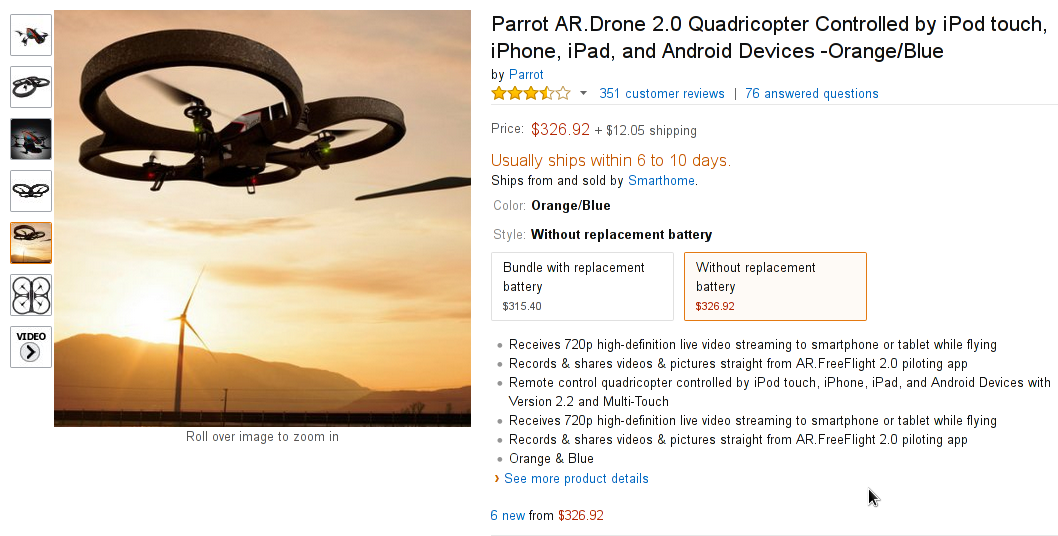
\includegraphics[scale=0.6]{img/ar_drone_2.png}
\end{center}





\end{document}
